\documentclass[twosided,a4paper]{article}           %type
\usepackage[top=2cm,bottom=2cm,inner=1.5cm,outer=1.5cm]{geometry}       %geometry
\renewcommand{\familydefault}{\sfdefault}


%\usepackage[italian]{babel}                %font/language
\usepackage[T1]{fontenc}
\usepackage[utf8]{inputenc}

\usepackage{amsmath}                       %maths
\usepackage{bm}
\usepackage{amssymb}					   %for numbersets

\usepackage{graphicx}
\usepackage{epstopdf} 
\usepackage{float}
\usepackage{subfigure}

\usepackage{tabularx}

%\usepackage{hyperref}

%\usepackage{subfloat}
%full packaging for image in eps finally
\usepackage{textcomp}

\usepackage{color}
\usepackage[dvipsnames]{xcolor}

\usepackage{listings} 

\newcommand{\tr}{^{\tiny{\bm \top}}}

\newenvironment{sistema}%
{\left\lbrace\begin{array}{@{}l@{}}}%
	{\end{array}\right.}

\begin{document}
	
	\title{\textcolor{MidnightBlue}{Mechanical vibration} - \textcolor{Plum}{System identification and modal analysis of 3-DOF linear system}}
	\author{Giammarco Valenti}
	\maketitle
	
\section{Dynamical system}

\subsection{The linear model}
The chosen model is a linear plant consisting of 3 masses, 3 springs between them, and 3 dampers between each mass and the ground. The model is shown in Figure \ref{fig:theplant1}.
\begin{figure}[H]
	\centering
	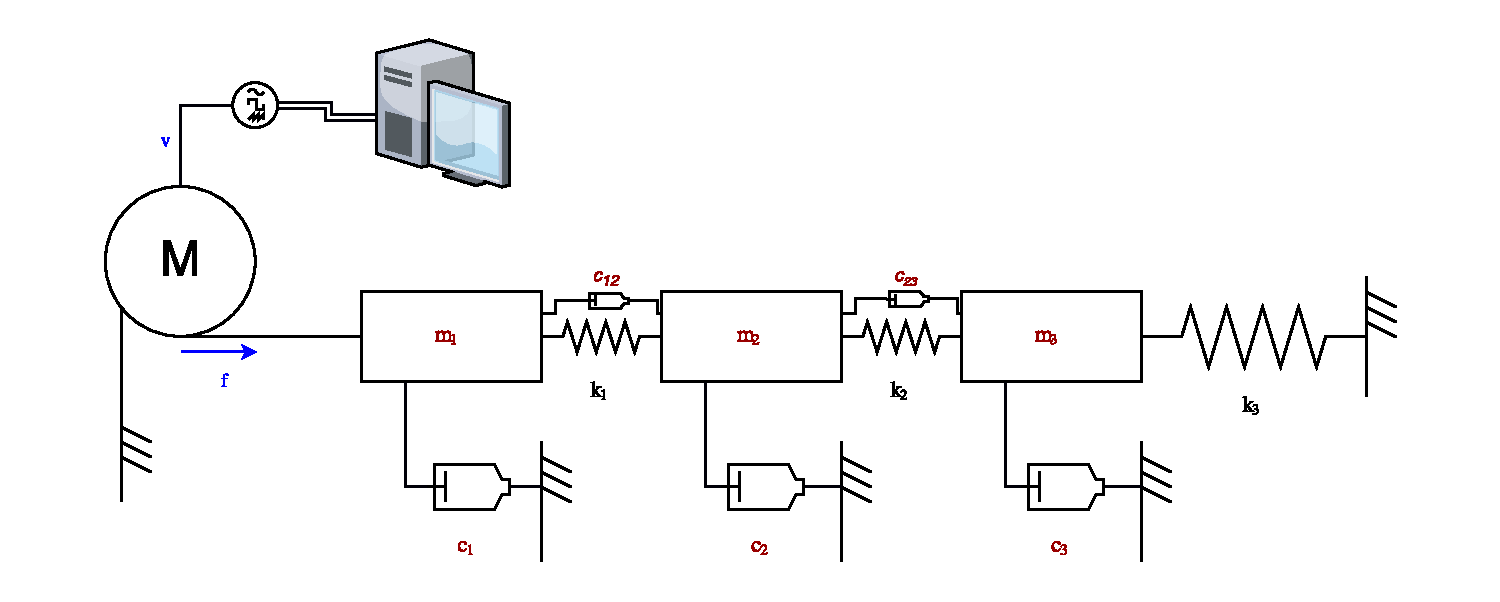
\includegraphics[width=\linewidth]{img/theplant1}
	\caption[The linear plant]{The chosen plant, in red the unknown parameters}
	\label{fig:theplant1}
\end{figure} %TODO figure with displacements x
\subsection{equation of motion}
\begin{equation}
	\begin{sistema}
	m_1 \ddot{x}_1 = + k_1 \left (x_2 - x_1 \right )                                 + c_{12} \left ( \dot{x}_2 - \dot{x}_1 \right )                                                  - c_1\dot{x}_1 + g_v v\\
	m_2 \ddot{x}_2 = + k_1 \left (x_1 - x_2 \right ) + k_2 \left (x_3 - x_2 \right ) + c_{12} \left ( \dot{x}_1 - \dot{x}_2 \right ) +  c_{23} \left ( \dot{x}_3 - \dot{x}_2 \right ) - c_2\dot{x}_2\\
	m_3 \ddot{x}_3 =                                 + k_2 \left (x_2 - x_3 \right )                                                 +  c_{23} \left ( \dot{x}_2 - \dot{x}_3 \right ) - c_3\dot{x}_3 - k_3 x_3
	\end{sistema}
\end{equation}
In the classical matrix form:
\begin{subequations}
\begin{equation}
	\bm M \ddot{x} + \bm C \dot{x} + \bm K x = \bm b
	\label{eq:eqm:tot}
\end{equation}
where:\\
	\begin{tabularx}{\linewidth}{@{}XXX@{}}
	\begin{equation}
\bm K = \left[ \begin{array}{ccc}
+ k_1  & - k_1 & 0 \\ 
-k_1 & + k_1 + k_2 & -k_2 \\ 
0 & - k_2 & + k_3
\end{array}  \right]
\label{eq:eqm:K}
\end{equation} &
	\begin{equation}	
		\bm M = \left [\begin{array}{ccc}
		m_1 & 0 & 0 \\ 
		0 & m_2 & 0 \\ 
		0 & 0 & m_3
	\end{array} \right ]
	\label{eq:eqm:M}
\end{equation} \\
	\begin{equation}
\bm b = \left[ \begin{array}{ccc}
g_v \\ 0 \\  0
\end{array}  \right]
\label{eq:eqm:b}
\end{equation} &
	\begin{equation}
	\bm C = \left[\begin{array}{ccc}
	+ c_1 + c_{12} & -c_{12} &  0 \\ 
	-c_{12} & +c_2 + c_{12} + c_{23} & -c_{23} \\ 
	0 & -c_{23} & c_3 + c_{23} 
	\end{array} \right]
	\label{eq:eqm:C}
	\end{equation}
	\end{tabularx}
\label{eq:Mtot}
\end{subequations}
\subsection{state-space model}
	The linear model of the plant, expressed by the equation \ref{eq:Mtot}, is a SIMO model. A state-space form was chosen to represent this model. The matrices are the follwing:\\
\begin{subequations}
\begin{tabularx}{\linewidth}{@{}XXX@{}}
	\begin{equation}
		A = \left [ \begin{array}{cc}
		\bm Z_{3 \times 3} & \bm I_{3 \times 3} \\ 
		\bm{-M^{-1}K} & \bm{-M^{-1}C}
		\end{array} \right ]
		\label{eq:ss:A}
	\end{equation} &
	\begin{equation}
	\bm B =	\left [ \begin{array}{c}
		\bm Z_{3\times 1} \\ 
		\bm{-M^{-1}b}
		\end{array} \right ]
		\label{eq:ss:B}
	\end{equation} \\
		\begin{equation}
	\bm C =	\left [\begin{array}{cc}
	\bm I_{3\times 3} & \bm Z_{3\times 3}
	\end{array}   \right ]
	\label{eq:ss:C}
	\end{equation} &
	\begin{equation}
	\bm D =	\left [\begin{array}{c}
	\bm Z_{3 \times 1}
	\end{array}   \right ]
	\label{eq:ss:D}
	\end{equation} 
\end{tabularx}
\end{subequations}
where $\bm I$ is the identity matrix and $\bm Z$ is a matrix with all the entries equal to zero.
\subsection{experimental setup}
\subsubsection{data processing}
Few operations on data must be performed in order to use them. At first, the data on diplacements is provided in \textit{encoder counts}. They are converted in meters with the following convertion factor ($g_x$):
\begin{equation}
	g_x = \dfrac{\Delta x}{\Delta \texttt{counts}} = 2 \pi r_e \cdot \dfrac{\Delta \texttt{counts}}{16000\dfrac{\texttt{counts}}{\texttt{encoder revolution}}}
\end{equation}
	\subsection{parameters and data available}

\subsection{initial hypothesis and approximations}
\begin{itemize}
	\item neglected motor electrical dynamics (instantaneous transmission of torque)
	\item rectilinear motion (all perfect aligned)
	\item inertia and damping of the motor are merged respectively into $m_1$ and $c_1$.
	\begin{equation}
	\begin{sistema}
		m_1 = m_{block} + \frac{J_{motor}\vert_{zz}}{r^2}\\
		c_2 = c_{block} + \frac{c_{motor}}{r^2}
	\end{sistema}
	\end{equation}
	where $r$ is the radius of the gear-rack coupling (gear wheel), $J_{motor}\vert_{zz}$ is the inertia of the motor , $c_{motor}$ the rotational damping and ''block'' quantities are the ones stricly related to the physical first mass.
	\item The term $c_3$ contains the viscous friction with the ground and the one due to the spring. In the model those two contributions cannot be quantified separately.
	
\end{itemize}
\section{System identification}
	
\subsection{step response analysis}
First of all, the step response analysis can be performed. In this analysis the ''static'' coefficients can be estimated, they are:
\begin{itemize}
	\item voltage to force $g_v$
	\item springs' stiffness $k_i$ with $i \in 1,2,3$
\end{itemize} 
The coefficient to be estimated is the \textcolor{Plum}{\textit{voltage-to-force}} coefficient %TODO SYMBOL 
\begin{equation}
	f = \textcolor{Plum}{\bm{(k_a\cdot k_t \cdot k_{mp})}}v = \textcolor{Plum}{g_v} v
\end{equation}.
In order to estimate the parameters the static gain vector $g_{dc}$ of the system has to be computed. The standard procedure is to apply the ''CAB'' formula from the state space formulation:
\begin{equation}
	\bm{g_{dc}} =	\bm{CA^{-1}B}
\end{equation}
which is the transfer function at $s = 0$. Since this computation implies the inverse of the $6 \times 6$ matrix $\bm A$, another computation is performed. Using the formulation in Equation \ref{eq:Mtot}, we can perform the following limits:
\begin{equation}
	\begin{sistema}
	\lim_{t \to + \infty}{\dot{x}}  = 0  \\
	\lim_{t \to + \infty}{\ddot{x}} = 0
	\end{sistema}
	\label{eq:dot_limits}
\end{equation}
The substitution \ref{eq:dot_limits} in \ref{eq:eqm:tot} yields:
\begin{equation}
\bm K x = \bm b
\label{eq:dot0}
\end{equation} The static gain is then:
\begin{equation}
	\bm{g_{dc}} = \bm{K^{-1}}\bm{b}
\end{equation}
Note that it is equivalent to apply the Laplace tranform to the equation \ref{eq:eqm:tot} and apply the final value theorem to it.
\begin{equation}
	\bm{g_{dc}} =
	\left [ \begin{array}{ccc}
	g_v\dfrac{k_1k_2 + k_3k_2 + k_3k_1}{k_1k_2k_3}  & g_v\dfrac{k_2+k_3}{k_2k_3} & g_v\dfrac{1}{k_3}
	\end{array} \right ]\tr
	\label{eq:g_dc}
\end{equation}
Note that in equation \ref{eq:g_dc} is evident from the expression the parallel between the stiffnesses (at steady state inertia and damping are invisible).
The steady state value of the three output are available. Some other computations has to be made to make equation \ref{eq:g_dc} suitable for the check on the stiffnesses ratios and the new estimation of $g_v$. The equation for the steady state values is:
\begin{equation}
	\bm{C}\bm{x}_\infty = \bm{g_{dc}}u_\infty  
	\label{eq:stst1}
\end{equation}
Where the $\infty$ denotes the steady state value of the quantity. The Equation \ref{eq:stst1} is now expressed in terms of stiffnesses ratio: $k_3$ is fixed to the nominal value and two ratio are defined:\begin{itemize}
	\item fix $k_3$ on nominal value
	\item multiplied both sides times $k_3$
	\item replace $R_{32} = \dfrac{k_3}{k_2}$
	\item replace $R_{31} = \dfrac{k_3}{k_1}$
\end{itemize}
This operations are made in order to make the system easy to solve, and uncoupling the nonlinear factor $g_v$. This allow to make to solve the system in a cascade fashion from $g_v$ to $R_{13}$. The equation \ref{eq:stst1} is now expressed in the following form:
\begin{equation}
	\label{eq:stst2} 
	k_3 \left [\begin{array}{c}
	x_1(\infty) \\ 
	x_2(\infty) \\ 
	x_3(\infty) \end{array}  \right ] 
	=
	u(\infty)\left [\begin{array}{c}
	g_v + g_v R_{13} + g_v R_{23} \\ 
	g_v R_{23} \\ 
	g_v \end{array}  \right ] 
\end{equation}
Now the next step is to use the measured value of steady state response (input and output), take $g_v$ as new estimated value and verify that $R_{12}$ and $R_{32}$ matches the nominal values. As set before $u(\infty) = 0.5$.
Results on the ratios are shown in Table \ref{tab:ratios}
%TODO< write the mambo jambo
\begin{table}[H]
	\centering
	\begin{tabular}{|c|c|c|c|}
		\hline 
		 & from data & nominal & error \% \\ 
		\hline 
		$k_3/k_2$ & \input{result/R32_exp.txt}& \input{result/R32_nom.txt} & \input{result/R32_per.txt}\%  \\ 
		\hline 
		$k_3/k_1$ & \input{result/R31_exp.txt}& \input{result/R31_nom.txt} & \input{result/R31_per.txt}\% \\
		\hline \hline
		      & from data              & initial & error 
		      \%\\
		\hline
		$g_v$ & \input{result/g_v.txt} & \input{result/gain_v.txt} & \input{result/g_v_per.txt}\% \\\hline
	\end{tabular} 
	\label{tab:ratios}
	\caption{Stiffnesses ratios and voltage-to-force coefficients results}
\end{table}
The $voltage-to-force$ estimation is shown in table \ref{tab:ratios}.
\subsection{Parameters estimation}

\begin{subequations}
\begin{equation}
	ciao
\end{equation}
\begin{equation}
	ciaone
\end{equation}
\end{subequations}

\end{document}